\documentclass[aspectratio=169]{beamer}
\usepackage[T1]{fontenc}
\usepackage[utf8]{inputenc}
\usepackage{listings}
\usepackage{colortbl}
\usepackage[scaled=.92]{helvet}
\renewcommand*\sfdefault{cmss}
\usepackage[sfmath]{kpfonts}

\definecolor{codegreen}{rgb}{0,0.6,0}
\definecolor{codegray}{rgb}{0.5,0.5,0.5}
\definecolor{codepurple}{rgb}{0.58,0,0.82}
\definecolor{backcolour}{rgb}{0.95,0.95,0.92}

\title{Kowalski - Your Helpful \\AI Assistant}
\author{Christian Goll <\texttt{cgoll@suse.com}>}
\date{\today}
\usetheme{suse}

\begin{document}
\begin{frame}
  \titlepage
\end{frame}

\begin{frame}{Outline}
  \tableofcontents
\end{frame}

\section{Introduction}
\begin{frame}[fragile]{The Challenge: LLMs and System Configuration}
\begin{columns}
\column{0.5\textwidth}
  \begin{block}{Current state}
    \begin{itemize}
      \item Large Language Models (LLMs) are powerful for general tasks.
      \item LLMs are allready used for system configuration tasks
      \item Halucinations and wrong tools likely to be presented
    \end{itemize}
  \end{block}
\column{0.5\textwidth}
  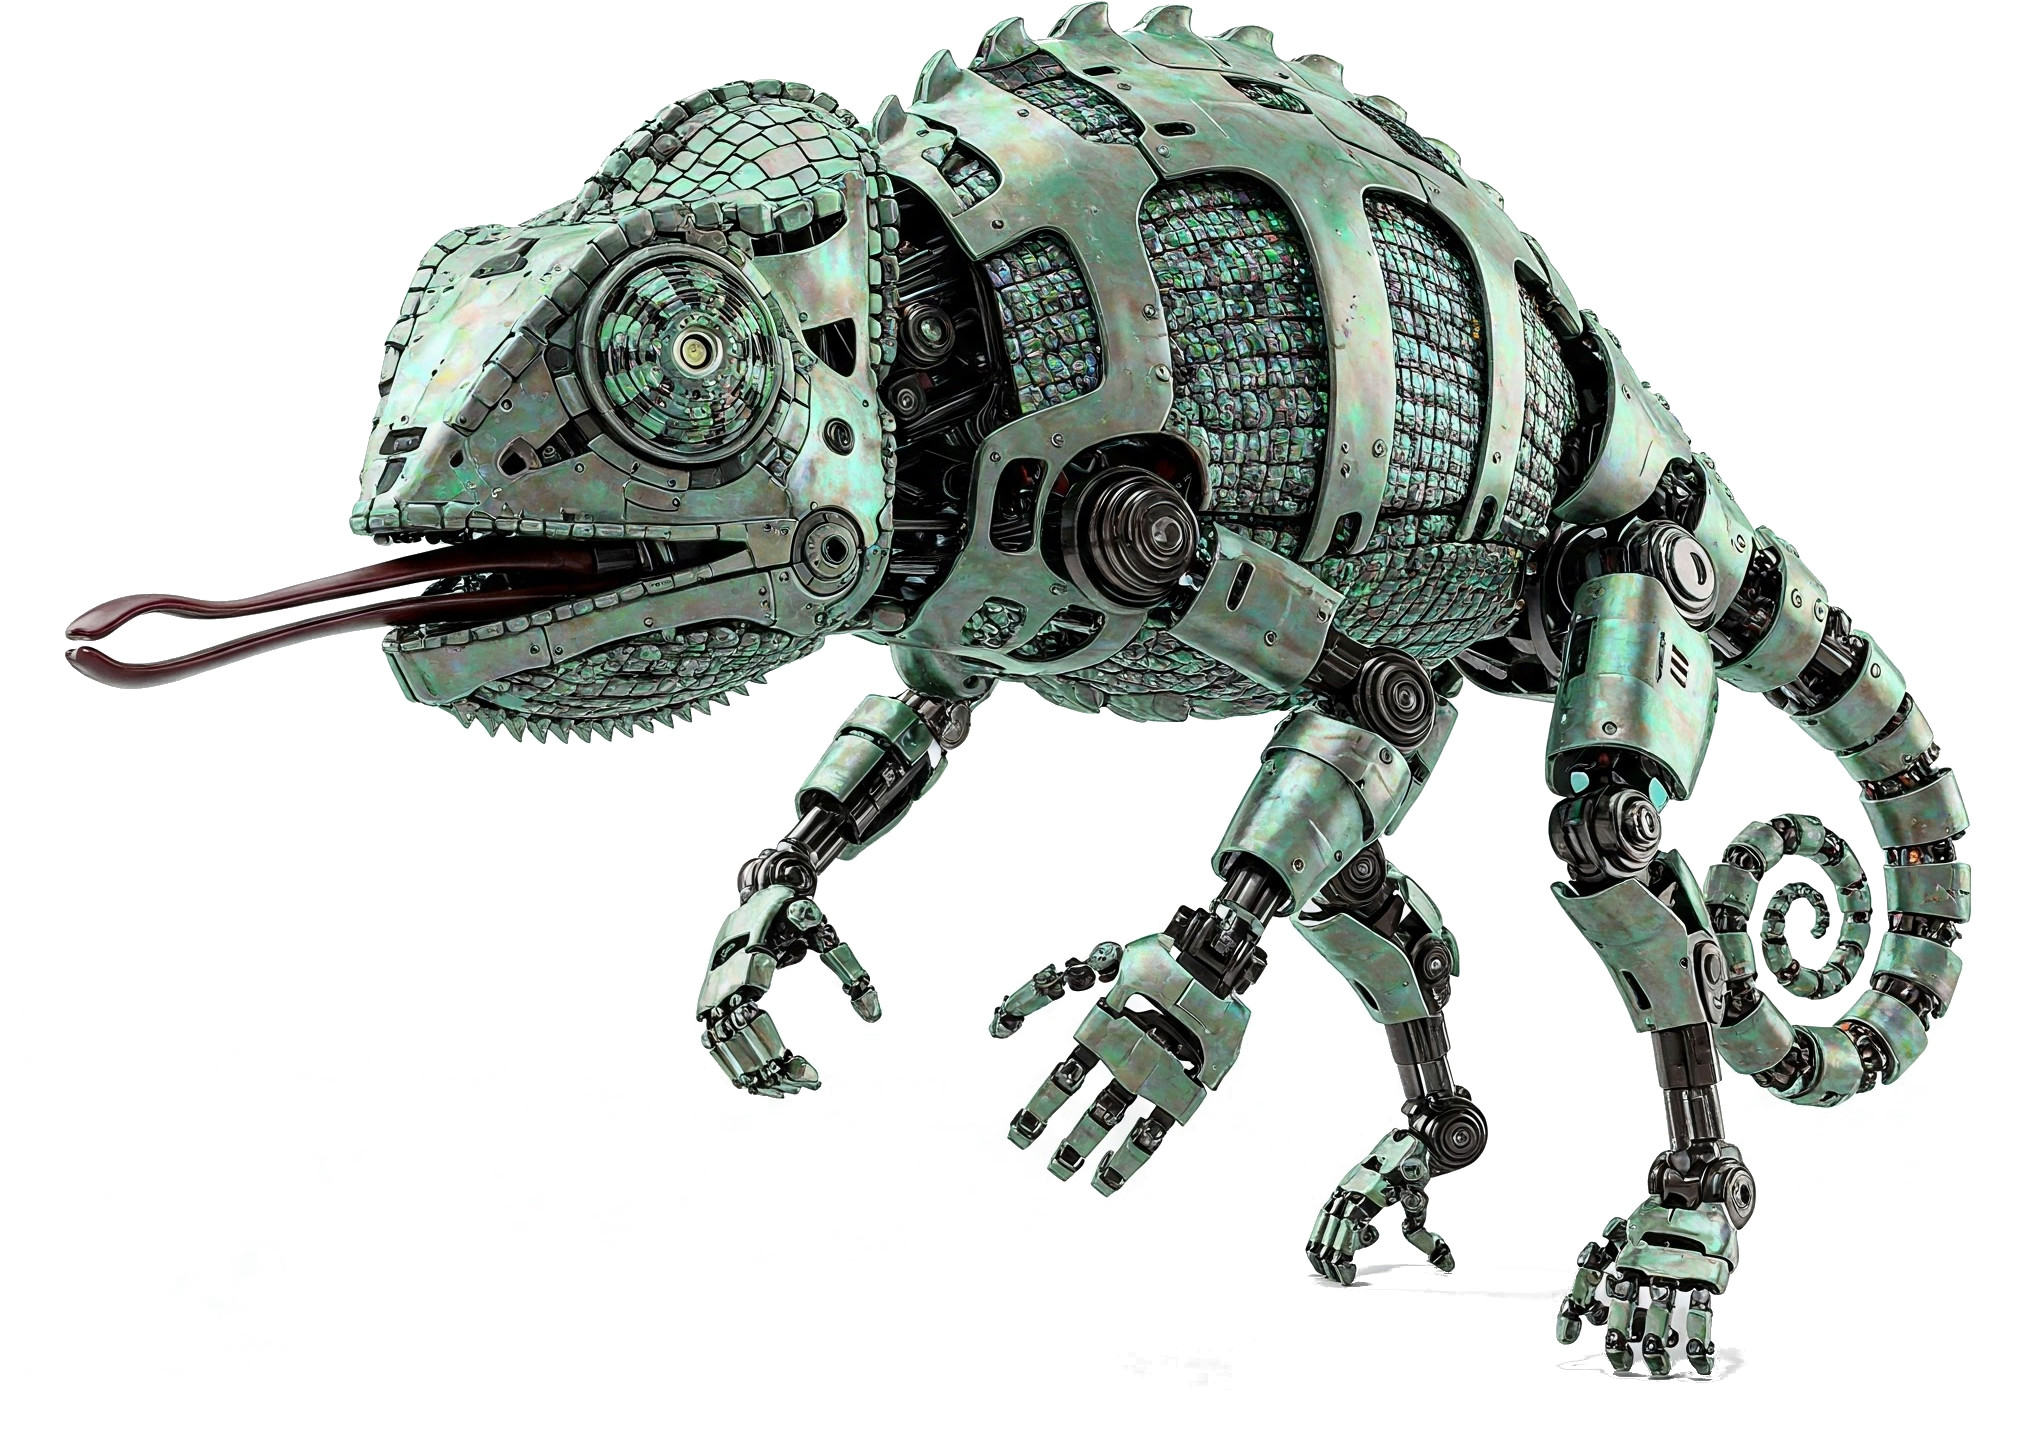
\includegraphics[width=\linewidth]{RobotChameleon}
\end{columns}
\end{frame}

\begin{frame}[fragile]{Example}
\begin{columns}
\column{0.5\textwidth}
\begin{itemize}
  \item Answers with standard prompt are extensive
  \item User has to select the right one
  \item Sensitive information may be shared!
\end{itemize}
\column{0.5\textwidth}
  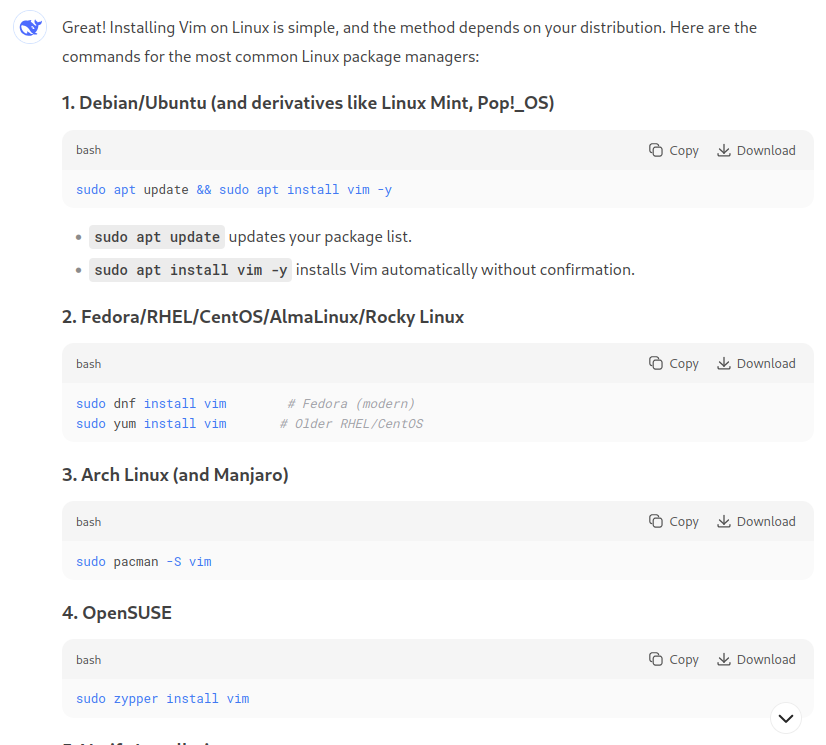
\includegraphics[width=\linewidth]{DeepSeek}
\end{columns}
\end{frame}

\begin{frame}[fragile]{Problem}
\begin{columns}
\column{.5\textwidth}
\begin{itemize}
  \item LLMs are created by training text completion on scraped sources
  \item LLMs don't have any context
\end{itemize}
\column{.5\textwidth}
  
\includegraphics[width=\linewidth]{JohnSnow}
\textbf{You know nothing, John Snow!} 
\end{columns}
\end{frame}

\begin{frame}[fragile]{Solution}
\begin{columns}
\column{.5\textwidth}
\begin{itemize}
  \item Context is needed for accurate solutions
  \item Should be easy to get context of actual system.
\end{itemize}
\column{.3\textwidth}
  
\includegraphics[width=\linewidth]{Tyrion}
\textbf{I know things!}
\end{columns}
\end{frame}

\section{Introducing Kowalski}
\begin{frame}{Introducing Kowalski: A Specialized AI Assistant}
\begin{columns}
\column{.5\textwidth}
  \begin{itemize}
    \item Kowalski is designed to bridge the gap between LLMs and system configuration.
    \item It provides LLMs with highly relevant and context-aware information.
    \item Focus on extracting and utilizing knowledge from technical documentation, specifically SUSE/SLE docs.
  \end{itemize}
\column{.3\textwidth}
  
\includegraphics[width=\linewidth]{Kowalski}
\end{columns}
\end{frame}

\begin{frame}{Excurse: Vector Embeddings}
  \begin{block}{Definition}
  Numerical representations of data (words, texts, etc.) in a vector space
  \end{block}
  \begin{block}{Key Properties}
  \begin{itemize}
    \item Capture semantic relationships \\(e.g., "king" – "man" + "woman" ≈ "queen").
    \item Fixed-length (e.g., 300 dimensions for Word2Vec).
    \item Similar items cluster together in the vector space.
  \end{itemize}
  \end{block}
  \begin{block}{Example}
  \texttt{"cat" → [0.2, -0.5, 0.7], "dog" → [0.3, -0.4, 0.6]}
  \end{block}
\end{frame}

\begin{frame}{How are Embeddings Created?}
  \begin{block}{Common Methods}
  \begin{description}
    \item[GloVe]\hfill \\ Uses global word co-occurrence statistics from a corpus.
    \item[Word2Vec (Skip-gram/CBOW)]\hfill \\Predicts surrounding words (or target word) using shallow neural networks.
  \end{description}
  \end{block}
  \begin{block}{Vector space search}
  \begin{itemize}
    \item Searching nearest neighbors in high dimesional vector space isn't  trivial
    \item Facebook created \texttt{faiss} library which does this job
  \end{itemize}
  \end{block}
\end{frame}

%------------------------------------------------
% Slide 4: Kowalski's Core Idea
%------------------------------------------------
\begin{frame}{Kowalski's Core Idea: Contextualized Information}
  \begin{itemize}
    \item Enhance the LLM's ability to perform configuration tasks.
    \item Achieve this by providing accurate information extracted directly from trusted sources (documentation).
    \item Supplement documentation knowledge with live system information.
  \end{itemize}
\end{frame}

%------------------------------------------------
% Slide 5: Phase 1: Documentation Ingestion
%------------------------------------------------
\section{Kowalski Workflow}
\begin{frame}{Phase 1: Documentation Ingestion}
  \begin{block}{The Starting Point: SUSE/SLE Documentation}
    \begin{itemize}
      \item Kowalski begins by processing official documentation.
      \item This documentation is a rich source of configuration knowledge.
      \item The goal is to make this information machine-readable and easily retrievable.
    \end{itemize}
  \end{block}
\end{frame}

%------------------------------------------------
% Slide 6: Extraction Process
%------------------------------------------------
\begin{frame}{Extraction Process: Identifying Key Information}
  \begin{columns}
    \column{0.5\textwidth}
    \begin{block}{What is Extracted?}
      \begin{itemize}
        \item Mentioned files (e.g., configuration files, scripts).
        \item Commands to be executed (e.g., installation, configuration commands).
        \item Key parameters and values within documentation examples.
      \end{itemize}
    \end{block}
    \column{0.5\textwidth}
    \begin{block}{How is it Extracted?}
      \begin{itemize}
        \item Utilizing parsing techniques.
        \item Applying Natural Language Processing (NLP) to identify relevant entities.
        \item Defining patterns and rules to capture structured information.
      \end{itemize}
    \end{block}
  \end{columns}
\end{frame}

%------------------------------------------------
% Slide 7: Building the Knowledge Base
%------------------------------------------------
\begin{frame}{Building the Knowledge Base: Internal Database}
  \begin{itemize}
    \item Extracted files, commands, and related documentation snippets are stored.
    \item An internal database is created to organize this structured information.
    \item This database serves as a central repository of documentation-derived knowledge.
  \end{itemize}
\end{frame}

%------------------------------------------------
% Slide 8: Semantic Understanding: Creating Embeddings
%------------------------------------------------
\begin{frame}{Semantic Understanding: Creating Embeddings}
  \begin{itemize}
    \item Embeddings are created from the documentation content.
    \item These embeddings capture the semantic meaning of the text.
    \item This allows for searching based on concept and relevance, not just keywords.
  \end{itemize}
\end{frame}

%------------------------------------------------
% Slide 9: The User Interaction
%------------------------------------------------
\section{User Interaction}
\begin{frame}{The User Interaction: Asking Kowalski}
  \begin{block}{User Query}
    \begin{itemize}
      \item A user poses a question to Kowalski regarding a system configuration task.
      \item The query is the starting point for retrieving relevant information.
    \end{itemize}
  \end{block}
\end{frame}

%------------------------------------------------
% Slide 10: Query Embedding
%------------------------------------------------
\begin{frame}{Query Embedding: Understanding the User's Need}
  \begin{itemize}
    \item The user's query is also converted into an embedding.
    \item This puts the query into the same semantic space as the documentation embeddings.
    \item Enables comparing the user's request to the stored knowledge.
  \end{itemize}
\end{frame}

%------------------------------------------------
% Slide 11: Finding Relevant Information: Vector Search
%------------------------------------------------
\begin{frame}{Finding Relevant Information: Vector Search with FAISS}
  \begin{itemize}
    \item FAISS (Facebook AI Similarity Search) is used for efficient vector similarity search.
    \item The embedding of the user query is compared against the documentation embeddings.
    \item The nearest (most semantically similar) help documents are identified.
  \end{itemize}
\end{frame}

%------------------------------------------------
% Slide 12: Enriching the Context
%------------------------------------------------
\begin{frame}{Enriching the Context: Adding System Specifics}
  \begin{block}{Going Beyond Documentation}
    \begin{itemize}
      \item The extracted relevant documentation snippets are a primary source of context.
      \item Kowalski then checks if files mentioned in the documentation exist on the *actual* system.
      \item The content of these existing system files is extracted.
    \end{itemize}
  \end{block}
\end{frame}

%------------------------------------------------
% Slide 13: The Enriched Context for the LLM
%------------------------------------------------
\begin{frame}{The Enriched Context for the LLM}
  \begin{itemize}
    \item The LLM receives a context that includes:
    \item Relevant information from the documentation (extracted text).
    \item Information about specific files found on the user's system that were mentioned in the documentation.
    \item This provides the LLM with a much more accurate picture of the user's situation.
  \end{itemize}
\end{frame}

%------------------------------------------------
% Slide 14: How it Works Together: The Kowalski Workflow
%------------------------------------------------
\begin{frame}{How it Works Together: The Kowalski Workflow}
  \begin{enumerate}
    \item Documentation Ingestion \& Extraction
    \item Database Creation \& Embedding Generation
    \item User Query
    \item Query Embedding
    \item Vector Search (FAISS)
    \item Retrieve Relevant Docs
    \item Check for Mentioned System Files
    \item Extract System File Content
    \item Provide Enriched Context to LLM
    \item LLM Generates Configuration Advice
  \end{enumerate}
\end{frame}

%------------------------------------------------
% Slide 15: Benefits of Using Kowalski
%------------------------------------------------
\section{Benefits}
\begin{frame}{Benefits of Using Kowalski}
  \begin{itemize}
    \item **Accuracy:** LLM responses are grounded in trusted documentation.
    \item **Relevance:** Context is tailored to the specific documentation and the user's system.
    \item **Efficiency:** Users get direct answers for configuration tasks.
    \item **Reduced Hallucination:** Providing specific context minimizes the risk of incorrect information.
    \item **Improved LLM Performance:** LLMs can provide more helpful and actionable configuration steps.
  \end{itemize}
\end{frame}

% End of document
\end{document}
